\section{Applicazioni di rete}
Abbiamo tutti a che fare ogni giorno con applicazioni che sfruttano internet:
\begin{itemize}
    \item il web
    \item la posta elettronica
    \item messaggistica istantanea
    \item social network
    \item trasferimento di file e trasferimento di file p2p
\end{itemize}

Creare una applicazione di rete significa creare dei programmi che devono essere eseguiti su macchine diverse che comunicheranno tra di loro attraverso la rete.
In genere si scrive software solo per gli host in quanto i dispositivi che compongono il network-core usano lo stack fino al livello network, quindi a loro non interessa il protocollo applicativo.
Vedremo che per alcune applicazioni ciò non è necessariamente vero.

\subsection{Architetture per le applicazioni}
Come già discusso riconosciamo 2 architetture principali per le applicazioni di rete: Client/Server e p2p, in alcuni casi tuttavia risulta più conveniente implementare un misto delle due.

\subsubsection{Server}
E' una macchina che deve essere sempre accesa in quanto deve sempre fornire il servizio, deve avere un indirizzo IP permanente perché se cambiasse bisognerebbe ricomunicarlo, per scalare bisogna costruire complesse infrastrutture di rete dette \emph{server farm}.

\subsubsection{Client}
Un client è una macchina che richiede il servizio, è un host intermittente in quanto si connette quando deve utilizzare il servizio e basta, può avere un IP che cambia col tempo.
I client non comunicano direttamente tra di loro, comunicano solo con il server!

\subsubsection{Peer}
In una rete peer-to-peer pura non c'è necessità di un "server" sempre attivo e connesso perché se vi sono altri peer collegati possono agire loro da server.
I componenti di questa rete comunicano tra di loro direttamente.
Possono connettersi arbitrariamente, possono cambiare IP.
E' una architettura largamente scalabile ma difficile da gestire!

Non c'è una vera e propria differenza tra client e server, spesso un host svolge il ruolo di entrambi.

\subsubsection{Architettura Ibrida}
Talvolta risulta più comodo implementare una applicazione in maniera ibrida, un esempio è skype: l'applicazione usa una connessione client/server per autenticare gli utenti e distribuire gli indirizzi IP dei partecipanti ma quando si avvia una chiamata tra due utenti la connessione è peer to peer.

Le reti p2p possono avere delle limitazioni come l'asimmetricità della connessione utilizzata e la sicurezza, alcune volte le architetture ibride possono risolvere alcuni dei problemi.

\subsection{Comunicazione tra processi}
Un processo è un programma in esecuzione, dati due processi sullo stesso host essi possono comunicare attraverso vari metodi messi a disposizione dal sistema operativo detti \emph{inter-process communication}. Un esempio è l'utilizzo di memoria comune o delle pipe.
Dati due processi su macchine diverse la comunicazione può avvenire solo attraverso la rete tramite lo scambio di messaggi.

Un processo client è un processo che inizia una comunicazione.

Un processo server è un processo che rimane in attesa di essere contattato.

\subsubsection{Application Programming Interface}
Per fare ciò i sistemi operativi moderni ci mettono a disposizione delle interfacce utilizzabili per implementare le applicazioni di rete senza preoccuparci di tutto ciò che c'è ai livelli inferiori.

In particolare si usano le \emph{socket-based API}, sono una struttura che mima le, già esistenti, caselle postali.

\begin{figure}[H]
    \centering
    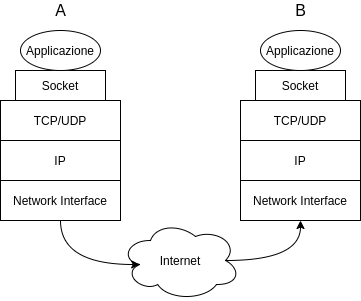
\includegraphics[width=250px]{images/2_Applicazioni_di_rete/socket.png}
\end{figure}

Queste API ci permettono di scegliere quale protocollo di trasporto usare e di configurare alcuni altri piccoli parametri ma di tutto il resto non dovremo preoccuparci minimamente.

\subsubsection{Come scegliere il protocollo di trasporto?}
Le API ci mettono a disposizione 2 protocolli di livello trasporto tra i quali scegliere.
La scelta va ovviamente fatta ponderando le caratteristiche della applicazione, in particolare:
\begin{itemize}
    \item \emph{reliability} - affidabilità: alcune applicazioni tollerano la perdita di informazioni o che l'arrivo delle informazioni non sia nello stesso ordine con il quale sono state inviate (streaming audio/video), per altre applicazioni è importante che i dati arrivino tutti e nell'ordine corretto (file transfer, chat)

    \item \emph{timing} - tempestività: alcune applicazioni hanno necessità che i dati arrivino in maniera veloce (VoIP, streaming), per altre applicazioni un piccolo delay non è importante
    
    \item \emph{throughput}: alcune applicazioni necessitano la garanzia di un minimo di velocità della rete (streaming in diverse qualità), per altri la velocità non è importante (file transfer, email)
    
    \item \emph{security}: per alcune applicazioni sono importanti gli aspetti della sicurezza, dell'integrità dei dati e della loro autenticità, per altre meno
\end{itemize}
I protocolli tra i quali scegliere sono:
\begin{table}[H]
    \centering
    \begin{tabular}{p{150px}|p{150px}}
        \multicolumn{1}{c}{\textbf{TCP}} & 
        \multicolumn{1}{c}{\textbf{UDP}}\\
        \hline        
        Orientato alla connessione, quindi si esegue un setup iniziale prima di poter trasmettere i dati &
        Non ha meccanismi di connessione \\
        \hline
        E' affidabile & 
        Non è affidabile, i pacchetti possono non arrivare o arrivare corrotti\\
        \hline
        Applica un controllo del flusso in modo da non sovraccaricare il ricevente &
        Nessun meccanismo di controllo del flusso \\       
        \hline
        Applica un controllo della congestione, se nota che la rete si avvicina ad una congestione cala drasticamente il  rate dei pacchetti & 
        Nessun meccanismo di controllo del flusso \\
        \hline
        Non fornisce timing, né security, né un throughput minimo &
        Non fornisce timing, né security, né un throughput minimo \\
        \hline
        Spesso chiamato \emph{stream} perché i pacchetti sono correlati l'uno con l'altro &
        Chiamato \emph{datagram} perché ogni pacchetto è da intendere singolarmente, spesso chiamato anche \emph{best effort} \\
    \end{tabular}
\end{table}

\subsection{Definizione di un protocollo applicativo}
Per definire un protocollo applicativo è necessario definire:
\begin{itemize}
    \item Il tipo dei messaggi scambiati: le richieste e le risposte
    \item La sintassi dei singoli messaggi: i campi di cui si compongono, come sono delineati
    \item La semantica del messaggio: il significato dei singoli campi, come vanno letti
    \item Le regole su quando e come i processi inviano e rispondono ai messaggi
\end{itemize}

Alcune di queste specifiche sono di dominio pubblico attraverso i documenti \emph{RFC}, questo si fa per permettere l'interoperabilità attraverso diverse macchine e diversi sistemi operativi. Alcuni di questi sono anche approvati in maniera ufficiale come HTTP e SMTP, altri sono solo definiti ma senza approvazione come BitTorrent.
Altri protocolli invece sono proprietari e quindi non hanno una documentazione ufficiale, ad esempio Skype.

\subsection{Indirizzamento dei processi}
Abbiamo detto che in una rete l'host è identificato da un indirizzo numerico a 32 bit detto indirizzo IP, ogni host può tuttavia eseguire diversi processi, serve quindi un metodo per indirizzarli singolarmente attraverso la rete.
Questo è possibile attraverso un altro numero di 16 bit detto \emph{numero di porta}.
Si dice quindi che un processo è in ascolto su una porta.

\subsection{HTTP}
Il protocollo HTTP è quello utilizzato per navigare il web.
Una pagina web consiste in vari oggetti che possono essere semplici pagine HTML, immagini JPEG, file audio e molto altro.
Quando si contatta un web server si scarica sempre una pagina web che poi ha le indicazioni per arrivare a tanti altri oggetti, questi indirizzi sono detti \emph{Uniform Resource Locator - URL}, per esempio: \emph{http://www.someschool.edu/someDept/pic.gif}, si compone di:
\begin{itemize}
    \item hostname: www.someschool.edu
    \item pathname: someDept/pic.gif
\end{itemize}

E' un protocollo client-server in cui il client è costituito dal browser che richiede e renderizza gli oggetti scaricati mentre il server accoglie le richieste ed invia le risorse richieste.
Usa TCP come protocollo di trasporto, di default usa la porta 80 e sfrutta i messaggi HTTP per formare le richieste.

E' un protocollo \emph{stateless} quindi ogni richiesta è a se stante ed il server da solo non è capace di correlare le diverse richieste l'una con l'altra: questo è comodo in quanto il protocollo è più semplice da implementare, non ci sono politiche di \emph{riconciliazione} dello stato qualora uno dei due dovesse essere corrotto e si limita l'uso della memoria.

\subsubsection{Persistent mode}
HTTP può essere:
\begin{itemize}
    \item Non persistente: viene scambiato al massimo un oggetto per connessione TCP
    \item Persistente: sono permessi più scambi di oggetti sulla stessa connessione TCP
\end{itemize}
E' chiaro che la versione persistente permette di diminuire le attese e l' uso della rete in quanto si risparmiano tutti i pacchetti necessari per instanziare la connessione TCP e per terminarla.

\subsubsection{Formato del messaggio}

La struttura di un messaggio di richiesta è il seguente:
\begin{figure}[H]
    \centering
    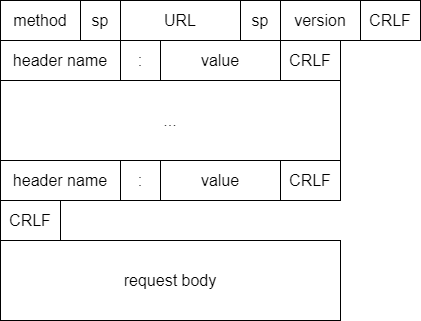
\includegraphics[width=300px]{images/2_Applicazioni_di_rete/HTTP_request.png}
\end{figure}
per esempio:
\begin{verbatim}
    GET /somedir/page.html HTTP/1.1
    Host: www.someschool.edu
    User-Agent: Firefox/15.0
    Connection: close
    Accept-language: it
\end{verbatim}

I metodi fondamentali messi a disposizione sono:
\begin{itemize}
    \item GET: usato dal client per richiedere le risorse
    \item POST: usato dal client per inviare dati, permette di inserire dati nel body
\end{itemize}

Un esempio di risposta è:
\begin{verbatim}
    HTTP/1.1 200 OK
    Connection close
    Date: Wed, 06 Aug 2013 12:00:15 GMT
    Server: Apache/1.3.0 (Unix)
    Last-Modified: Sun, 22 Jun 2013
    Content-Length: 6821
    Content-Type: text/html
    
    data ...
\end{verbatim}

Il protocollo permette di trasmettere eventuali errori tramite gli status header, la prima riga della risposta, composto da un numero (200) e dal significato canonico (OK).

Alcuni RFC che descrivono il protocollo sono:
\begin{itemize}
    \item \href{https://datatracker.ietf.org/doc/html/rfc1945}{1945}
    \item \href{https://datatracker.ietf.org/doc/html/rfc2068}{2068}
    \item \href{https://datatracker.ietf.org/doc/html/rfc2616}{2616}
    \item \href{https://datatracker.ietf.org/doc/html/rfc7230}{7540}
\end{itemize}

\subsubsection{Cookies}
Sono un metodo per rendere stateful il protocollo HTTP.
Quasi tutti i siti usano i cookies per mantenere informazioni attraverso le varie richieste.
Il meccanismo si compone di 4 componenti:
\begin{itemize}
    \item header cookie nella risposta
    \item header cookie nella richiesta
    \item file sul client che mantiene i cookie in memoria
    \item database del sito web che mantiene i dati associati al cookie
\end{itemize}
Il meccanismo funziona in questo modo:
\begin{itemize}
    \item il client esegue una normale richiesta
    \item il server risponde alla richiesta aggiungendo un header Set-Cookie con il nome del cookie, il valore ed altre informazioni utili
    \item alle prossime richieste il client provvederà ad inviare i cookie verso il server come "autenticazione"
    \item il server risponderà con normali risposte
\end{itemize}
All' interno dei cookie l' applicazione può memorizzare:
\begin{itemize}
    \item informazioni utili all' autenticazione
    \item scelta della policy dei cookies
    \item lingua scelta
    \item token della sessione
\end{itemize}

\subsubsection{Web cache - Proxy}
Se visitiamo spesso gli stessi siti è inutile contattare il server ogni volta, magari il server è anche lontano e quindi bisogna fare molta strada per contattarlo.
Per risolvere questo problema ed ottenere un miglioramento generale possiamo pensare di inserire un server nel mezzo tra il client ed il server ed utilizzarlo come una cache.

Una cache è una copia di un dato più vicino al computer e quindi più velocemente contattabile.
Un cache server si comporta sia da client (quando scarica la pagina dal server vero), sia da server (quando lo contattiamo per ottenere i dati copiati).
E' solitamente installata dagli ISP per ridurre il traffico nella rete.

\begin{figure}[H]
    \centering
    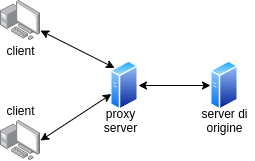
\includegraphics[width=220px]{images/2_Applicazioni_di_rete/cache_example.png}
\end{figure}
Il primo client richiede una risorsa, il proxy server se la procura, quando il secondo client chiede la stessa risorsa il proxy ce l' ha già e gliela fornisce direttamente.

La copia in cache potrebbe tuttavia essere vecchia, per risolvere questo problema è stato introdotto il \emph{conditional GET}, quando il proxy riceve una richiesta contatta il server di origine facendo una normale richiesta ed aggiungendo l'header:
\begin{verbatim}
    If-modified-since: <date>
\end{verbatim}
se il server vede che l' oggetto non è cambiato dalla data comunicata risponde con:
\begin{verbatim}
    HTTP/1.0 304 Not Modified
\end{verbatim}
se invece l' oggetto è stato cambiato si ottiene:
\begin{verbatim}
    HTTP/1.0 200 OK
    <data>
\end{verbatim}
con, appunto, la nuova copia dell' oggetto richiesto.


\subsection{FTP}
FTP sta per File Transfer Protocol, era un protocollo largamente utilizzato per lo scambio di file prima che HTTP esistesse.
E' ancora utilizzato per alcuni tipi di trasferimento come ad esempio per la gestione di spazi web o condivisione di file anonimi.
E' un protocollo client/server che permette di caricare file e scaricare file, quindi scambiare file in entrambe le direzioni.

Usa di default la porta 21 ed è specificato nell' RFC 959.
L' alternativa moderna è quella di utilizzare SFTP che è una versione di FTP che gira sulla porta 22 e prevede il traffico criptato.

Si basa su TCP per avere affidabilità ed una volta avviata la connessione ci si autentica con username e password.
Questa prima connessione sulla porta 21 è detta \emph{di controllo}, permette alcuni comandi come:
\begin{itemize}
    \item ls: elenca i file presenti nella cartella corrente
    \item cd: permette di cambiare la cartella di lavoro
    \item get: permette di scaricare un file
    \item put: permette di caricare un file
\end{itemize}

Usando i comandi get e put il server apre una connessione sulla porta 20, una volta connessi su quella porta possiamo avviare lo scambio del file.
Questa seconda connessione è detta \emph{dei dati}.
Alla fine del trasferimento si chiude questa seconda connessione.
La connessione di controllo rimane aperta per tutto il tempo e può anzi essere utilizzata per inviare altri comandi.

Possiamo quindi dire che:
\begin{itemize}
    \item la connessione di controllo è persitente
    \item la connessione dei dati non è persistente
\end{itemize}

Abbiamo due connessioni diverse perché se facessi tutto con la stessa connessione non potrei lanciare altri comandi nel frattempo.

La connessione di controllo è \emph{out of band} proprio per questa separazione dei canali.

FTP è stateful perché mantiene la directory corrente una volta effettuata l' autenticazione ed anche i file caricati continuano a rimanere sul server per la prossima connessione.

\subsection{Posta elettronica}
La posta elettronica è uno dei primi utilizzi di internet sin dalla nascita, si basa su 2 componenti principali:
\begin{itemize}
    \item \emph{user agent}: programma client usato per inviare e ricevere le mail, alcuni esempi sono elm, Mozilla Thunderbird, ecc.
    
    \item \emph{mail server}: programma server che mantiene in memoria la \emph{mailbox} dell' utente, cioè il contenitore dei messaggi in ingresso e la \emph{coda messaggi} cioè i messaggi in uscita.
    Si basa sul protocollo SMTP che si occupa di eseguire lo scambio delle email tra i diversi server mail.
    Ogni mail server che dialoga tramite SMTP è sia client, quando inizia la connesione per inviare la nuova mail, che server, quando riceve la connessione per ricevere le mail.
\end{itemize}

\subsubsection{SMTP - Simple Mail Transfer Protocol}
Il protocollo SMTP usa TCP per avere uno scambio affidabile, usa di default la porta 25 ed è testuale.
Supponiamo che lo user agent carichi direttamente la mail sul proprio mail server, ora questa mail deve arrivare al mail server del destinatario.
Il mail server guarda il destinatario e trova il mail server associato, inizia una connessione TCP, esegue l' handshake, tramite le regole del protocollo provvede ad inviare la mail e poi esegue una chiusura.
Il server mail al quale ci si connette risponde tramite degli status code e delle frasi, un po' come HTTP.
\begin{verbatim}
    S: 220 hamburger.edu
    C: HELO crepes.fr
    S: 250 Hello crepes.fr, pleased to meet you
    C: MAIL FROM: <alice@crepes.fr>
    S: 250 alice@crepes.fr... Sender ok
    C: RCPT TO: <bob@hamburger.edu>
    S: 250 bob@hamburger.edu ... Recipient ok
    C: DATA
    S: 354 Enter mail, end with "." on a line by itself
    C: Do you like ketchup?
    C: How about pickles?
    C: .
    S: 250 Message accepted for delivery
    C: QUIT
    S: 221 hamburger.edu closing connection
\end{verbatim}

SMTP usa connessioni persistenti, come HTTP, tuttavia SMTP è più un protocollo push in quanto si occupa prettamente di caricare dei dati mentre HTTP è principalmente pull in quanto sono più i download che gli upload.
SMTP usa CRLF.CRLF come terminatore di un messaggio ed invia più oggetti attraverso messaggi multipart cioè spezzettati in diversi pacchetti.

Il formato di un messaggio è:
\begin{figure}[H]
    \centering
    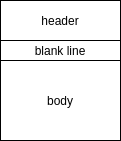
\includegraphics[width=80px]{images/2_Applicazioni_di_rete/messaggio_smtp.png}
\end{figure}
Alcuni esempi di header sono:
\begin{itemize}
    \item To
    \item From
    \item Subject
\end{itemize}
che sono diversi dai comandi SMTP!

Il body invece contiene il messaggio in soli caratteri ASCII.

Sappiamo che alle email possiamo aggiungere degli allegati non per forza testuali ma il protocollo ammette solo un body testuale.
Per avere questa feature altri due RFC sono stati creati: 2045 e 2046.
Questi documenti definiscono l'uso del MIME - Multipurpose Internet Mail Extensions, si tratta di due header aggiuntivi:
\begin{itemize}
    \item Content-Transfer-Encoding: specifica la codifica utilizzata per inviare il file (es: base64)
    \item Content-Type: specifica il tipo di file che si sta inviando, è utile per permettere a chi riceve di eseguire varie azioni in base al tipo
\end{itemize}

\subsubsection{POP3 - IMAP - WebMail}
Lo user agent deve connettersi al mail server corrispondente per scaricare le inbox ed inviare i messaggi in uscita.
Il protocollo POP3 - Post Office Protocol inizia con una autenticazione e poi usa la modalità \emph{download-and-keep}, POP3 è stateless tra le varie sessioni.
IMAP - Internet Mail Access Protocol è molto simile a POP3 ma ha più feature, anche lui tiene i messaggi sul server senza cancellarli, permette anche di organizzare le email in cartelle, è stateful attraverso le sessioni in quanto mantiene un mapping tra i messaggi e le cartelle assegnate.

In fine c'è la Webmail, lo user agent è un browser e le email vengono inviate attraverso HTTP.

\subsection{DNS}
Ricordare gli indirizzi IP, seppure in notazione decimale puntata, è difficile alla lunga, ci viene molto più comodo memorizzare dei nomi.
Proprio per questo motivo esistono gli \emph{hostname} cioè dei nomi associati ad uno o più indirizzi IP.
La traduzione da un nome all'indirizzo associato è detta \emph{risoluzione} e di questo compito si occupa il protocollo DNS.

E' un protocollo applicativo basato su UDP per avere una forte responsività, usa la porta 53 di default.
Per registrare un proprio dominio ci si rivolge ad un \emph{registrar} e dietro compenso lui si occupa di aggiungere i record DNS necessari.
Il DNS fornisce anche altri servizi:
\begin{itemize}
    \item traduzione da hostname ad indirizzo IP

    \item host aliasing: traduzione da un hostname ad un altro detto \emph{canonico}.
    Es: www.iet.unipi.it $\xrightarrow{}$ info.iet.unipi.it

    \item mail server aliasing: traduce gli indirizzi email negli hostname dei server associati a quell' indirizzo.
    Es: bob@hotmail.com $\xrightarrow{}$ server-1.hotmail.com

    \item distribuzione del carico: in base alle richieste ottenute posso tradurre un hostname con un indirizzo IP o con un altro in modo da usare equamente tutti i mirror di un servizio.
    Per fare ciò il server DNS restituisce l'intero elenco di IP associati al dominio ma ogni volta ruota la lista in modo da farne comparire in alto uno diverso.
\end{itemize}

Per dare un ordine ed evitare che lo stesso hostname sia modificato da più enti diversi il DNS fa uso di un database \emph{gerarchico} e \emph{distribuito}.
Distribuito per evitare un single point of failure; un singolo server sovraccaricato di richieste, magari anche distante per alcuni host, in pratica non è facilmente \emph{scalabile}.

\subsubsection{Prima approssimazione}
Un client vuole risolvere www.amazon.com, esegue una query DNS al \emph{root server} per trovare il DNS server che si occupa dei domini .com.
Successivamente il client esegue una query su quel DNS per ottenere l' indirizzo del DNS server associato al dominio amazon.com.
In fine il client contatta questo ultimo server DNS per ottenere l' IP di www.amazon.com

I root name server sono 13 in tutto il mondo, ognuno dei quali poi è ridondato tramite altri mirror, questa distribuzione fa si che in media il tempo per contattare questi DNS sia uguale dappertutto (per guardare i root nameserver consultare \href{https://www.root-servers.org/}{www.root-servers.org}).

\subsubsection{TLD server}
Sono i server Top-Level-Domain cioè i server che si occupano di gestire tutti i domini che finiscono in .com, .org, .net e tutti i top level domain dei vari paesi come .it, .uk, .fr, ecc.

\subsubsection{Authoritative server}
Sono quei server DNS che si occupano di risolvere tutti i sottodomini sotto un dominio, in genere sono tenuti da organizzazioni e service provider.
Sono utili in una azienda per gestire i domini interni come mail, web, ecc.

\subsubsection{Local DNS server}
E' il server al quale gli host si rivolgono nella realtà, esegue la vera e propria traduzione contattando i diversi DNS server necessari e restituisce il risultato all' host che ha eseguito la query.
Solitamente è mantenuto dall' ISP ed agisce come un proxy implementando anche una cache.

\subsubsection{Risoluzione iterativa}
\begin{figure}[H]
    \centering
    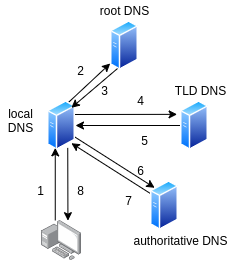
\includegraphics[width=200px]{images/2_Applicazioni_di_rete/risoluzione_DNS.png}
\end{figure}
Supponiamo che l' host richieda la risoluzione di www.unipi.it: esegue la sua query verso il suo local DNS, il local DNS contatta prima il root DNS per ottenere l' indirizzo IP del TLD DNS responsabile di .it, una volta avuto il suo indirizzo lo interroga per ottenere l' IP dell'authoritative DNS di unipi.it, in fine a lui chiede la risoluzione di www.unipi.it.

\subsubsection{Risoluzione ricorsiva}
\begin{figure}[H]
    \centering
    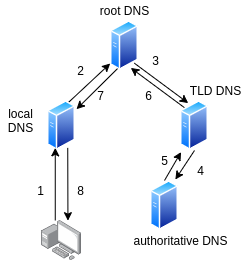
\includegraphics[width=200px]{images/2_Applicazioni_di_rete/risoluzione_DNS_ricorsiva.png}
\end{figure}
In questa configurazione ogni server contattato si occupa di risolvere interamente la query richiesta.
Tuttavia aumenta il carico sui server interemedi che generalmente sarebbero più liberi.

\subsubsection{Caching}
Ogni DNS server ha la propria cache, anche l' host stesso, il timeout delle entries è di solito 2 giorni.

In particolare i TLD DNS server sono cachati nel local DNS perché sono tante le richieste per lo stesso TLD.

\subsubsection{Record DNS}
La struttura di un record DNS è:
$$ (name, value, type, ttl) $$
il ttl è il Time-To-Live cioè il tempo per il quale il record è valido.
Esistono vari tipi di record DNS, i più comuni sono:
\begin{itemize}
    \item tipo A: name contiene l' hostname, value contiene l' IP

    \item tipo CNAME: name contiene l' alias per qualche nome, mentre value contiene il nome canonico

    Es: (www.hal.com, servereast.backup2.hal.com)

    \item tipo NS: name contiene il dominio, value contiene l' hostname dell' authoritative DNS per quel dominio
    
    Es: (hal.com, dns.hal.com)
    
    \item tipo MX (mail exchange): name contiene il dominio, value contiene il nome canonico del mailserver associato al dominio
\end{itemize}

\subsection{Distribuzione di file - comparazione tra C/S e p2p}
Quanto tempo serve per distribuire un file da 1 server ad N peer?
\begin{figure}[H]
    \centering
    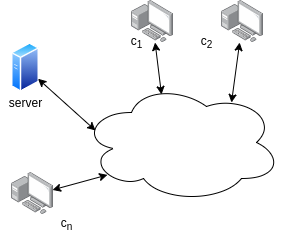
\includegraphics[width=220px]{images/2_Applicazioni_di_rete/distribuzione_file.png}
\end{figure}
Poniamo i seguenti dati:
\begin{itemize}
    \item $F$: dimensione del file
    \item $u_s$: velocità di upload del server
    \item $u_i$: velocità di upload del peer $i$
    \item $d_i$: velocità di download del peer $i$
\end{itemize}
Usando un' architettura client/server la velocità per scaricare un file può essere:
\begin{itemize}
    \item $\frac{NF}{u_s}$: tempo che serve al server per inviare il file a tutti
    \item $\frac{F}{d_i}$: tempo necessario al client per ricevere il file
\end{itemize}
In definitiva abbiamo:
$$ d_{cs} = max\{ \frac{NF}{u_s}, \frac{F}{d_i} \} $$
per $N \xrightarrow{} \infty$ il termine cresce in maniera lineare.

Usando un' architettura p2p la velocità per scaricare un file può essere:
\begin{itemize}
    \item $\frac{F}{u_s}$: prima copia
    \item $\frac{F}{min\{d_i\}_i}$: tempo per caricare il file nel nodo con velocità minore
    \item $\frac{NF}{\left( u_s + \sum u_i \right)}$: tempo per scaricare $N$ copie del file usado il massimo upload rate
\end{itemize}
Si noti che il terzo termine ha il denominatore che può essere assunto come $\left( u_s + Nu_{medio}\right)$ quindi:
$$ \frac{NF}{u_s + Nu_{medio}} \xrightarrow{N \xrightarrow{} \infty} \frac{F}{u_{medio}} $$
\begin{figure}[H]
    \centering
    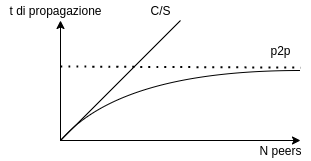
\includegraphics[width=200px]{images/2_Applicazioni_di_rete/comparazione_cs_p2p.png}
\end{figure}

\subsection{Ricerca di informazioni in una rete p2p}
Essendo una rete distribuita è necessario sapere dove trovare le risorse che si cercano.
Se un peer mette a disposizione dei file, un altro peer deve poter cercare e sapere cosa ha a disposizione.
Se parliamo di un protocollo di messaging invece è necessario conoscere l' IP accoppiato ad un username in modo da effettuare la connessione diretta.
Ci serve pertanto un indice nel quale effettuare le nostre query di ricerca.
Supponiamo quindi di dover creare un database i cui record sono formati da: (chiave, valore) in cui la chiave è il contenuto che vogliamo cercare ed il valore è l' IP del nodo che la possiede.
I peer dovranno poter eseguire query in questo database ed anche inserire delle entry in modo che possano essere utili agli altri.
Vediamo alcuni approcci.

\subsubsection{Centralized Index}
Il servizio di indicizzazione è offerto da uno o più server centralizzati, quando un nodo torna online lo notifica al server che provvede ad aggiornare il suo database, quando si esegue una query si contatta il server che risponde alla richiesta.
Siamo davanti ad un approccio ibrido in quanto l'indicizzazione e quindi la ricerca dei contenuti è client/server mentre lo scambio dei file o dei messaggi è p2p in quanto avviene tramite connessione diretta dei peer.

Un esempio di questa struttura è quella offerta da Napster che permetteva di cercare la musica presente nella rete p2p tramite il suo server centralizzato, ma poi il vero e proprio scambio avveniva in modalità p2p.

Questo approccio ha alcuni problemi:
\begin{itemize}
    \item costituisce un single point of failure, come qualsiasi servizio centralizzato
    \item potrebbe portare a problemi di performance in quanto tutte le richieste sono fatte allo stesso host
    \item la responsabilità del servizio in caso di problemi legali può essere attribuita a chi mantiene il server di indicizzazione
\end{itemize}

\begin{figure}[H]
    \centering
    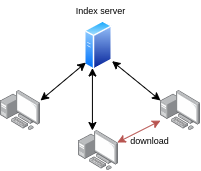
\includegraphics[width=200px]{images/2_Applicazioni_di_rete/centralized_index.png}
\end{figure}

\subsubsection{Query flooding}
E' un approccio completamente decentralizzato, usato dall' originale GNUtella.
L' indice è distribuito su tutti i nodi della rete che distribuiscono contenuti, i nodi sono connessi tra di loro a formare un gigantesco grafo.
Quando si deve eseguire una query di ricerca si forgia una richiesta e la si invia a tutti i propri nodi adiacenti: se loro hanno la richiesta risponderanno, altrimenti propagheranno la richiesta ai loro adiacenti e così via.
Si parla di \emph{flooding} proprio perché il numero di richieste che circola all' interno della rete è grandissimo. Se la rete diventa molto grande per problemi di scalabilità si può passare ad eseguire delle \emph{limited-scope query}: la propagazione viene eseguita un numero massimo di volte, per esempio dopo il terzo hop la richiesta non si ripete più.
Questo tuttavia può portare a dei falsi negativi: non troviamo la risorsa non perché non ci sia ma perché non siamo arrivati all' host che la fornisce.

\begin{figure}[H]
    \centering
    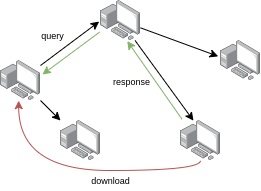
\includegraphics[width=250px]{images/2_Applicazioni_di_rete/query_flooding.png}
\end{figure}

Per costruire una rete del genere il protocollo GNUtella si serve di una lista di peer molto attivi, oppure di un server tracker che registra un insieme di IP di peer.
Quando un nuovo nodo vuole entrare a far parte della rete usa una di queste liste per ottenere alcuni IP di altri nodi, inizia dunque una connessione TCP ed invia un messaggio \emph{ping} con un campo \emph{peer-count} inizializzato ad un certo valore, ogni nodo che riceve questo ping lo ritrasmette ai suoi vicini decrementando peer-count fino ad arrivare a 0.
Qualsiasi host riceva questo ping risponde con un \emph{pong} in cui inserisce anche il proprio IP per permettere la connessione TCP.

\subsubsection{Hierarchical overlay}
E' una via di mezzo tra i due precedenti, utilizza dei nodi più importanti degli altri detti \emph{supernodi} per slegarsi da una centralizzazione ma non allarga troppo la lista dei peer che costruiscono l' indice.
Questi supernodi sono nodi con alta banda, con lunghi tempi online, sono connessi tra di loro a formare una seconda rete ed ognungo di loro contiene una porzione dell' indice che propaga agli altri.
I peer normali si connettono ai supernodi per informarli del loro contenuto e per eseguire le query di ricerca, una volta ottenuto il record di risposta si provvede ad una normale connessione p2p.

\begin{figure}[H]
    \centering
    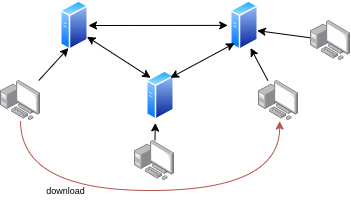
\includegraphics[width=280px]{images/2_Applicazioni_di_rete/hierarchical_overlay.png}
\end{figure}

\subsubsection{Distributed hash table}
E' un database p2p distribuito, usato da eMule.
Si assegna un identificatore di peer nel range [0, $2^{n-1}$], e le chiavi utilizzate sono nello stesso range.
Le chiavi sono ottenute passando la chiave di ricerca all' interno di una funzione di hash.
Le tuple (chiave, valore) sono associate ai peer in modo che ogni chiave sia associata al peer con l'ID più vicino ma maggiore, questo peer è chiamato \emph{successore immediato}.

Es: se $n = 4$ ed abbiamo i peer: [1, 3, 4, 5, 8, 10, 12, 14], la chiave 13 ha come immediato successore 14, la chiave 15 ha come immediato successore 1, ecc.

Ogni peer è a conoscenza solo del suo immediato successore e del suo predecessore, abbiamo di fatto una lista circolare.
Quando un nodo deve aggiungere un nuovo record o cercare tramite la chiave invia la richiesta al suo immediato successore e così via finché la tupla non raggiunge l' host con ID più vicino e maggiore, a quel punto il responsabile per quella chiave risponde direttamente tramite l' IP all' interno della richiesta.

Questa struttura impiega complessità $O(N)$ per eseguire una query, possiamo abbreviarla inserendo delle shortcut e permettendo quindi connessioni anche oltre all' immediato successore.
Si può quindi passare ad avere ogni nodo connesso a $O(logN)$ vicini, facendo scendere anche la complessità della richiesta a $O(logN)$.

Per gestire la scomparsa di un host dalla rete ogni peer oltre a conoscere il suo successivo conosce anche il successivo del successivo, periodicamente pinga i due successivi e se qualcuno è andato offline provvede a riconfigurare la sua posizione nell' anello.

\begin{figure}[H]
    \centering
    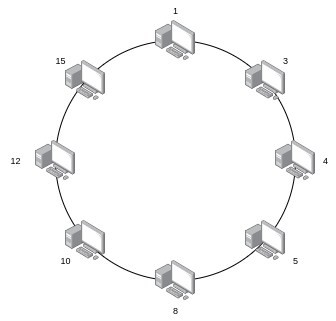
\includegraphics[width=200px]{images/2_Applicazioni_di_rete/DHT.png}
\end{figure}

\subsubsection{BitTorrent}
E' un protocollo di scambio di file che permette di scaricare da più peer contemporaneamente:
\begin{figure}[H]
    \centering
    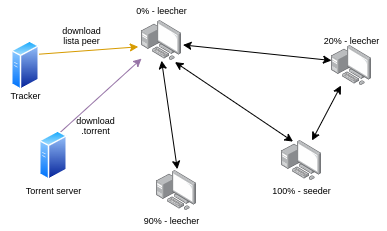
\includegraphics[width=250px]{images/2_Applicazioni_di_rete/bittorrent.png}
\end{figure}
I file da scambiare sono divisi in chunk da 256KB.
Ogni nodo della rete è un peer, ma può svolgere compiti diversi:
\begin{itemize}
    \item torrent server: è un server, spesso non facente parte della vera rete di distribuzione dei chunk, che mantiene in memoria i file .torrent e permette a chiunque di scaricarli.

    \item tracker: è un server che traccia i peer che fanno parte della rete di distribuzione di un torrent in modo da metterli in contatto tra di loro
    
    \item seeder: peer che ha completamente scaricato i file puntati dal torrent e continua a distribuirli
    
    \item leecher: peer che non ha ancora completato il download dei file, scarica i nuovi chunk ed allo stesso tempo carica i chunk che possiede
\end{itemize}

I file .torrent sono file che contengono informazioni sulla rete, in particolare l' IP del tracker e le informazioni sui chunk da cercare (hash dei blocchi in modo da non poterli sostituire arbitrariamente).

Quando si vuole entrare nella rete si contatta il tracker e si inizia una connessione con i peer inviati come risposta dal tracker.
Il trasferimento avviene in chunk quindi ad ogni istante ogni peer ha un certo numero di chunk.
Quando ci si connette agli altri peer, ed anche ad intervalli regolari, ci si scambia la lista dei chunk posseduti da ognuno in modo da decidere quale altro richiedere.
Quando si richiede non importa l' ordine perché tanto poi possono essere riordinati a posteriori, tuttavia si usa la metrica del \emph{rarest first}, cioè una volta chiesta la lista alle proprie connessioni si richiedono prima i chunk meno comuni, questo si fa per aumentare la presenza di questi chunk nella rete.

La scelta delle proprie connessioni è eseguita tramite la logica \emph{tit-for-tat} cioè si hanno 4 connessioni contemporaneamente con i 4 peer con il più alto rate di trasmissione.
Ogni 10 secondi si rivaluta questo gruppo ed ogni 30 secondi si sceglie casualmente un altro peer per iniziare a scambiare chunk. Questo per verificare se sia conveniente modificare i 4 migliori in questo momento: \emph{optimistically unchoke}.

\subsubsection{Skype}
Skype è un protocollo proprietario di messaggistica.
Ha una architettura a supernodi e l' indice mappa gli username agli IP.
Se i nodi sono dietro NAT per comunicare si usano i supernodi come relay per trasmettere il traffico.
E' un esempio di applicazione real-time.

\subsection{Socket}
Sono una interfaccia inizialmente costruita per BSD4.1 UNIX, nel 1981, usata per creare applicazioni di rete.
Sono strutture esplicitamente create, usate e rilasciate dalle applicazioni tramite chiamate a sistema.
Sfruttano un paradigma client/server ma sono abbastanza flessibili da poter creare anche applicazioni p2p.

Permettono di utilizzare 2 protocolli di trasporto:
\begin{itemize}
    \item quello a datagramma: UDP
    \item quello a stream: TCP
\end{itemize}
Dallo stesso socket una applicazione può ricevere ed inviare messaggi.
Oltre che attraverso la rete possono essere usati anche per inter-process comunication tra processi sulla stessa macchina.

Un socket è identificato da un indirizzo IP, quello della macchina che lo ha aperto, e da una porta, un numero identificativo richiesto dal programma stesso che gestisce il socket.
Per comunicare si usano due socket, uno per ogni endpoint della comunicazione.
